In the sequel, we detail the application of scPCA to a number of simulated and publicly available datasets, comparing our proposal to several competing techniques. An additional analysis of protein expression data is presented in Section \ref{sup_mice}. \edit{Details on hyperparameters used by all dimensionality reduction methods are presented in Sections \ref{sup_sim}, \ref{sup_dengue}, and \ref{sup_aml}.}

\subsection{Simulated scRNA-seq Data}\label{sim_scRNA-seq}

The scPCA technique was tested on a simulated scRNA-seq dataset generated with the \textit{Splat} framework from the \texttt{Splatter} \texttt{R} package  \citep{Zappia2017}. \textit{Splat} simulates a scRNA-seq count matrix by way of a gamma-Poisson hierarchical model. This simulation framework mimics real scRNA-seq data by including hyperparameters to control the number of over- and under-expressed genes (using multiplicative factors for mean expression levels), zero inflation, batch effects, and other technical and biological factors relevant for scRNA-seq data.

A simple dataset of 300 cells and 500 genes was simulated such that the cells were approximately evenly distributed among three biological groups: two groups making up a target dataset and a third group corresponding to a background dataset. 5\% of the genes are differentially expressed between the background dataset and each of the two target datasets but not between the two target datasets, 10\% of the genes are differentially expressed between the background dataset and the first target dataset but not the second target dataset, and 10\% of the genes are differentially expressed between the background dataset and the second target dataset but not the first target dataset. There is overlap between these three sets of genes and, in particular, a total of 98 genes are differentially expressed between the two target datasets. Based on these levels of differential expression, cells are more dissimilar between the two target datasets than between either of the target datasets and the background dataset. Therefore, the samples comprising the background dataset can be viewed as a set of controls for use by cPCA and scPCA. Additionally, a large batch effect was included to confound the biological variation between groups, effectively dividing each biological group into two subgroups of \edit{near} equal size (Figure~\ref{fig:sim}A).

\begin{figure*}[!htbp]
  \centering
  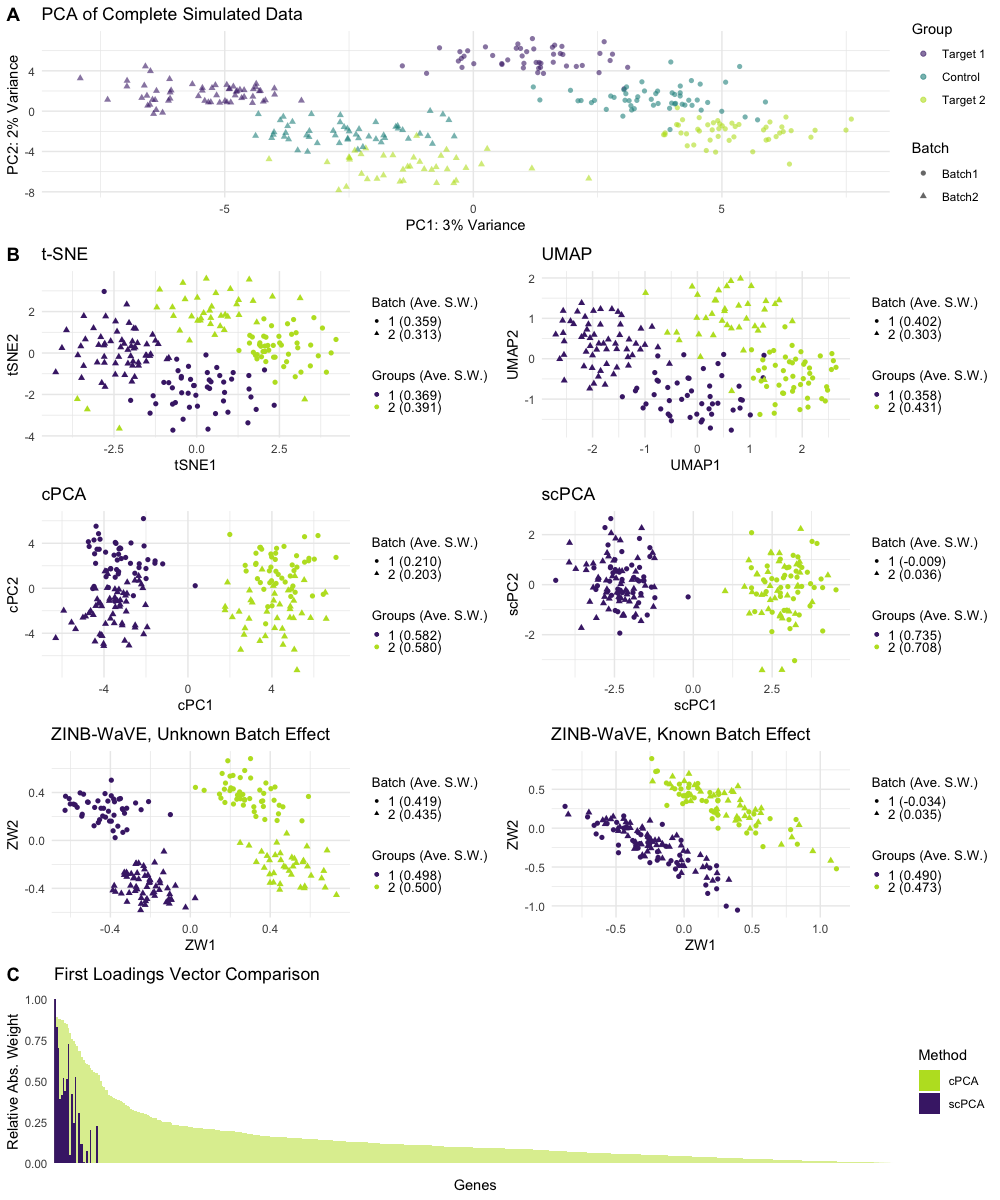
\includegraphics[width = \textwidth]{figures/sim_results}
  \caption{
  {\em Simulated scRNA-seq data.}
  \textbf{A} Plot of the first two principal components of the complete simulated dataset (i.e., the combination of the target and background datasets). The batch effect and the biological signal are responsible for approximately identical amounts of variance. \textbf{B} Two-dimensional representations of the target dataset by t-SNE, UMAP, cPCA, scPCA, and ZINB-WaVE, with accompanying average silhouette widths quantifying the strengths of the batch effect and the biological signal. Only scPCA fully removes the batch effect in two dimensions when batches are not adjusted for explicitly. \textbf{C} A gene-by-gene comparison of the \edit{standardized absolute loadings} in the first loading vectors of cPCA and scPCA, in decreasing order with respect to the values produced by cPCA.}
  \label{fig:sim}
\end{figure*}

PCA, t-SNE, UMAP, cPCA, and scPCA were applied to the log-transformed and column-centered target data\edit{, and SIMLR to the raw target data}, to determine whether these methods could identify the biological signal of interest, i.e., the two groups in the target dataset (Figure~\ref{fig:sim}B. Note that PCA was not included due to the similarity of results to Figure~\ref{fig:sim}A \edit{and SIMLR's embedding is included in the appendix in Figure~\ref{fig:simulated_SIMLR}}). Also note that cPCA was not performed in the traditional manner of \citet{Abid2018}, but with automatic hyperparameter selection as described in Sections \ref{hyp_tune} \edit{and \ref{algo1}}. The number of \textit{a priori} specified clusters for the cPCA and scPCA methods was set to 2, and the column-centered background data were used in their contrastive steps. While PCA, t-SNE, UMAP, \edit{SIMLR,} and cPCA were incapable of completely eliminating the batch effect in their two-dimensional representations, scPCA successfully removed the unwanted variation while producing the tightest clusters, as indicated by the average silhouette widths (see also Figure~\ref{fig:ave_sil_widths}), and generating sparse, interpretable loadings.

To compare the loadings produced by cPCA and scPCA, each of their loading vectors were standardized as follows. The $i^{\text{th}}$ entry of the $j^{\text{th}}$ standardized loading vector is given by 
$
\frac{|V_{ij}| - \text{min}_i |V_{ij}|}{\text{max}_i |V_{ij}| - \text{min}_i |V_{ij}|}
$, 
where $\mathbf{V}$ is a $p \times k$ loading matrix. 
Juxtaposing the \edit{standardized absolute loadings} of the first loading vectors produced by cPCA and scPCA, each of which linearly separate the target dataset's groups, we find the scPCA loadings to be, as expected, much sparser (see Figure~\ref{fig:sim}C). In fact, only 20 genes have non-zero values in scPCA's first loading vector compared to 500 in cPCA; moreover, these 20 genes correspond to those which have the largest absolute entries in cPCA's first loading vector. Furthermore, these genes are among the most differentially expressed in the target dataset, based on the values of their multiplicative differential expression factors (Figure~\ref{fig:sim_de_genes}).

scPCA's results were also compared to the two leading latent factors found by ZINB-WaVE, a method of choice for dimensionality reduction for scRNA-seq data, under conditions in which the batch factor is viewed as known and unknown (Figure~\ref{fig:sim}B). In both cases, ZINB-WaVE was applied to the count matrix of the simulated target dataset with no gene-level covariates. When the batch factor was treated as unknown, no cell-level covariates were included in the model; however, when we treated the batch factor as known, a binary cell-level covariate was added to indicate each sample's batch membership. When the batch effect is not explicitly regressed out in the ZINB-WaVE model, we find the results to be virtually identical to those of PCA. Even when the batch effect is included in the model, the clusters of the biological groups are elongated and less dense than those produced by scPCA, and the first latent factor does not linearly separate the groups.

\subsection{Dengue Microarray Data}\label{dengue_data}

\citet{Kwissa2014} used gene expression microarrays to analyze the whole-blood transcriptome of 47 dengue patients hospitalized at the Siriraj Hospital in Bangkok and 9 local healthy controls. Of the affected patients, 18 were classified as having acute dengue fever (DF), 10 as having acute dengue hemorrhagic fever (DHF), and 19 as convalescent at least four weeks after discharge.

As part of data pre-processing, all but the 500 most variable genes were filtered out. The target dataset consists of the log-transformed microarray expression measures of 47 patients with some form of dengue, while the background dataset consist of the log-transformed microarray expression measures of the control samples. PCA, cPCA, scPCA, t-SNE, and UMAP were then applied to the column-centered target data matrix with the goal of discerning three unique clusters (Figure~\ref{fig:dengue}A), one for each sub-class of dengue (DF, DHF, and convalescent). cPCA and scPCA took as additional input the column-centered background data matrix and specified three clusters \textit{a priori}. t-SNE's embedding was found to be similar to UMAP's and is therefore only included in the supplementary materials (Figure~\ref{fig:dengue_tsne}).

Of the four dimensionality reduction methods, only cPCA and scPCA successfully fully separated the convalescent patients from those with DF and DHF in two dimensions. scPCA's low-dimensional representation was virtually identical to that of cPCA, producing very similar average silhouette widths among classes, though only a tenth of the genes have non-zero values in the first and second columns of the scPCA loading matrix, and the most important genes identified by each methods' first loading vector differ substantially (Figure~\ref{fig:dengue}B). The genes found by scPCA include CD38, HLA-DQB1, and RSAD2 (Viperin), which have been previously associated to the susceptibility to, protection against, or presence of dengue \citep{Castaneda2016,Cardozo2014,Fitzgerald2011}. For a full list of these genes, refer to Table \ref{tab:dengue_1} and Table \ref{tab:dengue_2}. \edit{A gene set enrichment analysis (GSEA) was also performed with the genes contained in these tables to identify the most significant biological processes in which they play a role; details and results are presented in Table \ref{tab:gsea_dengue}.}

No method successfully distinguished between the three sub-classes of dengue. In fact, previous research suggests that the transcriptomes of patients with DF and DHF are virtually indistinct \citep{Kwissa2014}. Instead, \citet{Kwissa2014} found that DF and DHF patients may form distinct clusters based on viral load and concentration of the DENV NS-1 antigen in their plasma. This may explain the sub-clusters within the DF and DHF cases found by UMAP. Though the number of pre-specified clusters for each algorithm was set to three, cPCA's and scPCA's projections onto two dimensions contain two clusters. To test the sensitivity of these methods to this tuning parameter, both methods were reapplied to the data with varying numbers of pre-specified clusters. Each of cPCA's iteration produced virtually identical embeddings (Figure~\ref{fig:dengue_cpca_centers}). However, scPCA's produced identical results to those of PCA when the number of clusters was set to four or higher (Figure~\ref{fig:dengue_scpca_centers}). This may provide an empirical approach to selecting the appropriate number of clusters for scPCA, i.e., selecting the largest value before which the quality of the embedding deteriorates.

\FloatBarrier
\begin{figure*}[!htbp]
  \centering
  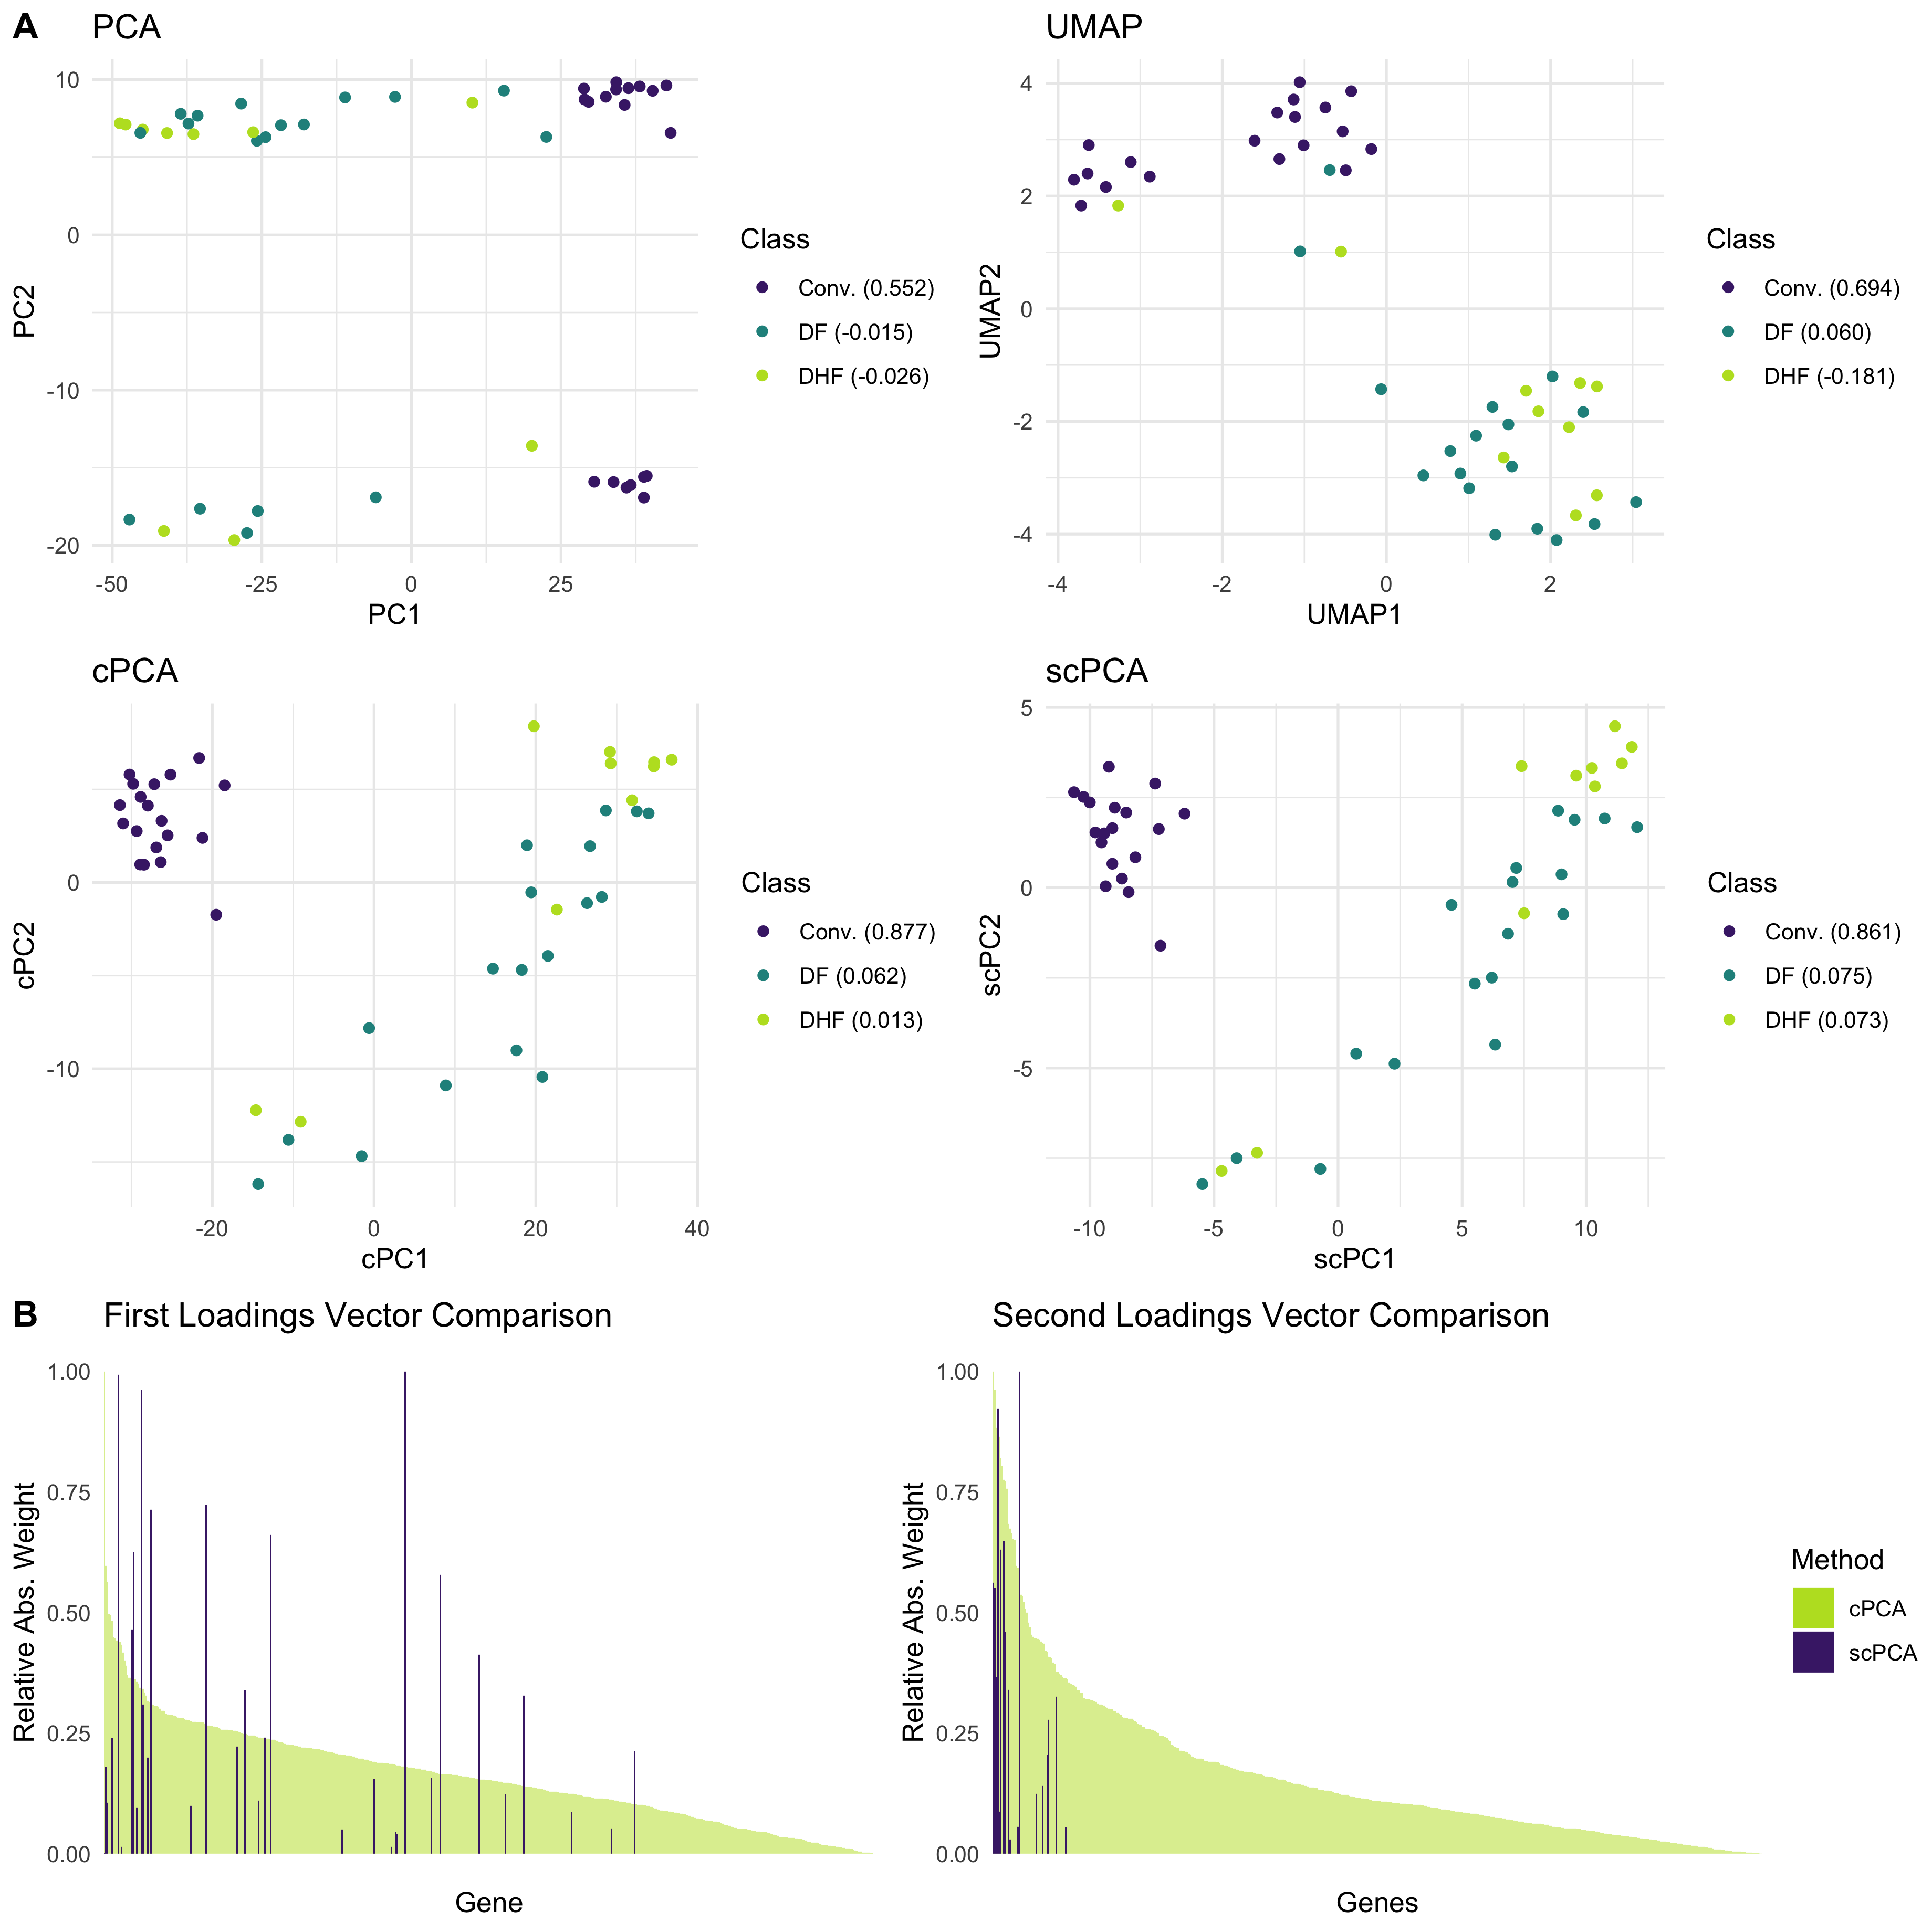
\includegraphics[width = \textwidth]{figures/dengue_results}
  \caption{
  {\em Dengue microarray data.}
  \textbf{A} Two-dimensional representations of the target dataset by PCA, UMAP, cPCA, and scPCA, with accompanying average silhouette widths quantifying the strengths of the biological signal.  cPCA and scPCA are the only methods that fully separate the convalescent patients from those with DF and DHF. The second PC of the PCA plot is dominated by some batch effect, and the low-dimensional representation produced by UMAP also appears to be affected by some source of unwanted variation. \textbf{B} The \edit{standardized absolute loadings} in the two leading loading vectors of scPCA are much sparser than those of cPCA, though their two-dimensional embeddings are virtually identical. The genes are in decreasing order of cPCA's \edit{standardized absolute loadings}, demonstrating that the genes with non-zero \edit{loadings} in scPCA generally correspond to the genes with the largest \edit{absolute loadings} in cPCA. This is much more apparent for the second loading vector where the distribution of cPCA's absolute loadings has a thin tail, attributing increased importance to a small subset of genes.}
  \label{fig:dengue}
\end{figure*}

\subsection{Leukemia Patient scRNA-seq Data}\label{leukemia_data}

Finally, we tested scPCA on scRNA-seq data from the cryopreserved bone marrow mononuclear cell (BMMC) samples of two acute myeloid leukemia (AML) patients (Patient 035: 4,501 cells; Patient 027: 7,898 cells), before and after undergoing allogeneic hematopoietic stem cell transplant treatment \citep{Zheng2017}. The BMMCs of two healthy individuals from the same publicly available dataset (Healthy 1: 1,985 cells; Healthy 2: 2,472 cells) were used to generate a control dataset. Following pre-processing, all but the 1,000 most variable genes measured across all 16,856 cells were removed. The scRNA-seq data from the AML patients were then split into separate target datasets since \citet{Zheng2017} found evidence of distinct subpopulation membership following transplantation. Data belonging to the healthy controls were combined to create the background dataset. PCA, t-SNE, UMAP, ZINB-WaVE, \edit{SIMLR,} cPCA, and scPCA were applied to the target datasets to explore differences in the AML patients' BMMCs's transcriptome engendered by the treatment (Figures~\ref{fig:comp_leuk_pat1},~\ref{fig:comp_leuk_pat2},\edit{~\ref{fig:SIMLR_aml_035}, and ~\ref{fig:SIMLR_aml_027}}).

Of the seven dimensionality reduction methods applied to Patient 035's data (Figures~\ref{fig:comp_leuk_pat1}A \edit{ and ~\ref{fig:SIMLR_aml_035}}), cPCA and scPCA best capture the biologically meaningful information relating to treatment status. Each produces linearly separable clusters corresponding to pre- and post-treatment cells; scPCA's projection yields a tighter cluster of pre-transplant cells when compared to that produced by cPCA, and the opposite is true regarding the clusters of post-transplant cells. Additionally, scPCA's projection required considerably less information, even though its results are analogous to cPCA's: 176 genes and 17 genes have non-zero entries in, respectively, the first and second columns of the loading matrix produced by scPCA (Figure~\ref{fig:comp_leuk_pat1}B). In general, the leading loading vectors of cPCA and scPCA place an increased importance on the same genes. \edit{Genes with non-zero \edit{loadings} in scPCA's first and second loading vectors were also subjected to a gene set enrichment analysis to uncover their roles in biological processes; details and results are presented in Table \ref{tab:gsea_aml035}}. Regarding the other methods' results, PCA, t-SNE, \edit{and SIMLR} fail to separate the pre- and post-transplant cells, and UMAP's and ZINB-WaVE's embeddings resemble a trajectory more closely than they do a set of clusters.

Similarly to Patient 035's results, the two-dimensional embeddings of Patient 027's data produced by PCA, t-SNE, UMAP, \edit{SIMLR,} and ZINB-WaVE do not contain distinct clusters of pre- and post-transplant BMMCs \ref{fig:comp_leuk_pat2}; however, cPCA and scPCA generate low-dimensional representations of the data in which samples are clustered based on treatment status. Although cPCA's representation produces denser\edit{, more distinct} groupings, the first two columns of scPCA's loading matrix contain non-zero values in only \edit{five} genes, STMN1, \edit{CA1, LDHA,} PDLIM1\edit{, and C1QBP. The first four genes have been linked to leukemia \citep{Machado-Neto2014,Mentese2017,Wang2014,Holleman2004}, and the last gene, C1QBP, is responsible for a protein that plays a critical role in tumor metabolism \citep{Fogal2010}.}

\FloatBarrier
\begin{figure*}[!htbp]
  \centering
  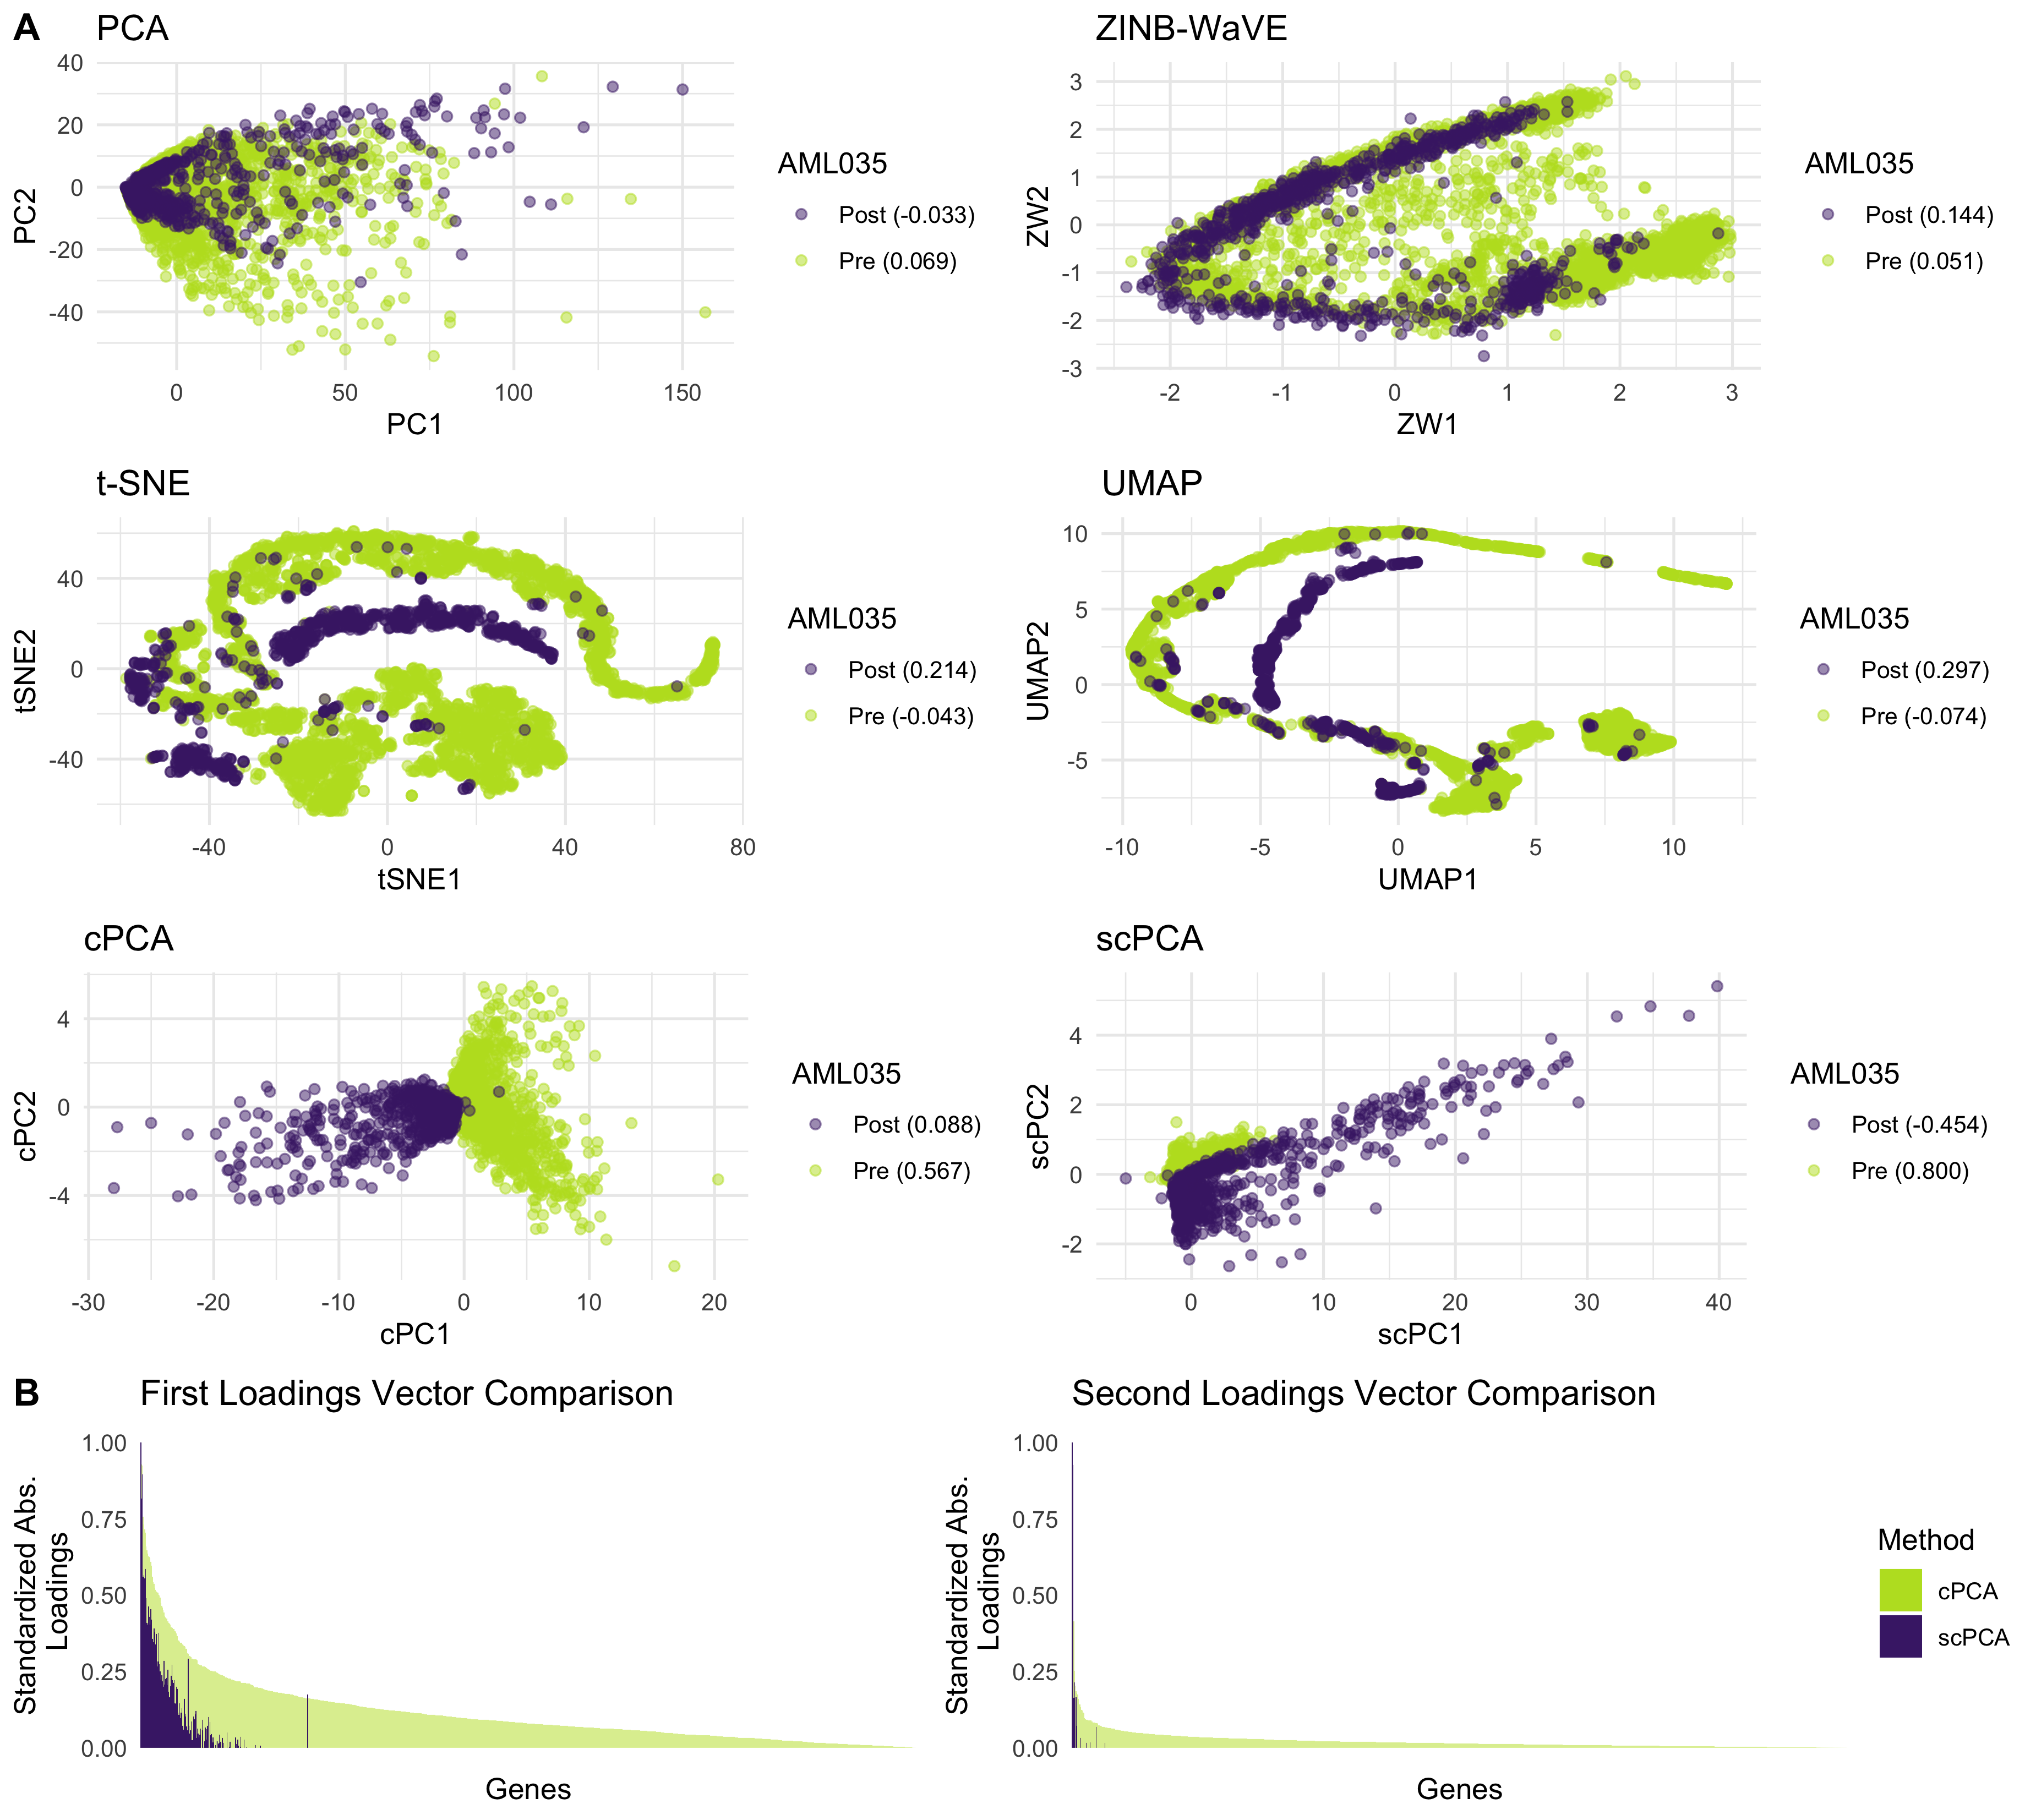
\includegraphics[width = \textwidth]{figures/aml035_results}
  \caption{{\em AML Patient 035 scRNA-seq data.} 
  \textbf{A} The two-dimensional embeddings of the patient's BMMCs produced by PCA, ZINB-WaVE, t-SNE, UMAP, cPCA, and scPCA, with accompanying average silhouette widths quantifying the strengths of the biological signal. cPCA and scPCA produce representations of the data in which the pre- and post-transplant cells form discernible clusters. Based on visual inspection and average silhouette width, scPCA's grouping of pre-transplant cells is denser than that of cPCA's and the opposite is true of the post-transplant cells' cluster. \textbf{B} scPCA's embedding is much sparser, increasing interpretability of the exploratory analysis.}
  \label{fig:comp_leuk_pat1}
\end{figure*}